\subsection{Smart Contract Security Analysis}

\subsubsection{Unauthorized Minting Prevention}

\textbf{1. Threat Model and Attack Vector}\\

In a decentralized academic certification ecosystem, the integrity of the entire platform relies heavily on the authenticity of the minting process \cite{blockchainineducation}. Because a minted Non-Fungible Token (NFT) represents an official, legally binding university degree \cite{fairfield2022tokenized}, the \texttt{mintCertificate(...)} function is the most critical and highly targeted entry point in the smart contract architecture \cite{perez2020smartcontracts}.\newline

An external malicious actor (attacker) or an unprivileged user could attempt to execute a direct contract transaction calling the \texttt{mintCertificate(...)} function by targeting the deployed contract address on the network \cite{rojalina2025verifichain}. The Attacker's Objective:

\begin{itemize}
    \item To bypass institutional verification gates and self-mint an unauthorized diploma \cite{khati2023studentcert}

    \item To dilute the trust of the academic registry by injecting fraudulent credentials into the ledger \cite{kumutha2021blockchainacdaemic}
\end{itemize}

Without rigorous access control mechanisms embedded directly into the smart contract state machine \cite{openzeppelin2026erc721}, any network entity possessing an EVM-compatible wallet address could broadcast a transaction containing arbitrary student metadata arrays, forcing the blockchain to anchor fake certificates permanently \cite{xiongfei2022nftcert}.\\

\textbf{2. Solution: Architectural Implementation of \texttt{onlyOwner}}\\

To neutralize this attack vector, the smart contract utilizes an explicit access control pattern inherited from OpenZeppelin's standardized security libraries [25]. By binding the onlyOwner modifier directly to the execution signature of the minting function, the platform establishes an immutable cryptographic boundary \cite{openzeppelin2026erc721}. The \texttt{onlyOwner} mechanism operates on a simple but absolute identity evaluation principle \cite{openzeppelin2026erc721}:

\begin{lstlisting}[
        language=solidity,
        style=codeStyle
    ]
    function mintCertificate(
        address student,
        string memory ipfsHash
    ) public onlyOwner returns (uint256) {
        // Minting execution logic only proceeds if msg.sender == owner
        return _executeMint(student, ipfsHash);
    }
\end{lstlisting}

During the contract compilation and initialization phase handled within the development suite \cite{hardhat2026ethereum}, the account address used to deploy the contract (the University Administrator's primary deployment key) is permanently recorded in the contract’s storage state as the \texttt{\_owner} \cite{onlinev0835web}. When any transaction triggers \texttt{mintCertificate(...)}, the EVM intercepts the instruction and executes an internal validation rule: \texttt{require(msg.sender == owner, "Ownable: caller is not the owner");} \cite{openzeppelin2026erc721}\cite{william2018eip721}. If the public key hashing the transaction signature (\texttt{msg.sender}) does not match the stored administrator address, the condition evaluates to false, immediately breaking execution \cite{perez2020smartcontracts}\cite{onlinev0835web}\\

\textbf{3. Result and State Reversion}\\

When an unauthorized entity initiates a call to \texttt{mintCertificate(...)}, the blockchain engine enforces an atomic rollback \cite{wood2008EthereumYellowPaper}.

\begin{itemize}
    \item \textbf{State Preservation}: The transaction fails completely \cite{yuan2014testing}. No new Token ID is generated, no IPFS metadata is bound \cite{benet2014ipfs}, and no state variables inside the MongoDB database mirror or the local Hardhat node are modified \cite{hardhat2026ethereum}.

    \item \textbf{Gas Consumption Penalties}: The attacker's transaction is forcefully marked as Status: Fail (Reverted) \cite{onlinev0835web}. All state modifications are completely rolled back as if the transaction never occurred, and the remaining execution gas is consumed, adding an economic penalty for the malicious actor \cite{onlinev0835web}\cite{wood2008EthereumYellowPaper}.

    \item \textbf{Error Logs}: The system emits a clear execution exception, typically logging Error: VM Exception while processing transaction: reverted with reason string 'Ownable: caller is not the owner' \cite{hardhat2026ethereum}.
\end{itemize}

\begin{figure}[H]
    \centering
    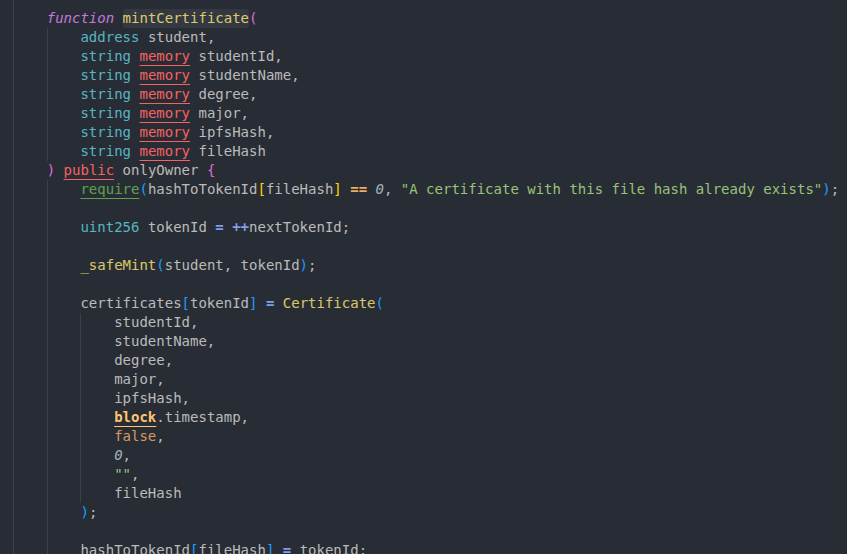
\includegraphics[width=0.85\textwidth]{images/mint_cert_func.png}
    \caption{minCertificate Function - Smart Contract Access Control Protection}
    \label{fig:mint_cert_func}
\end{figure}

\begin{figure}[H]
    \centering
    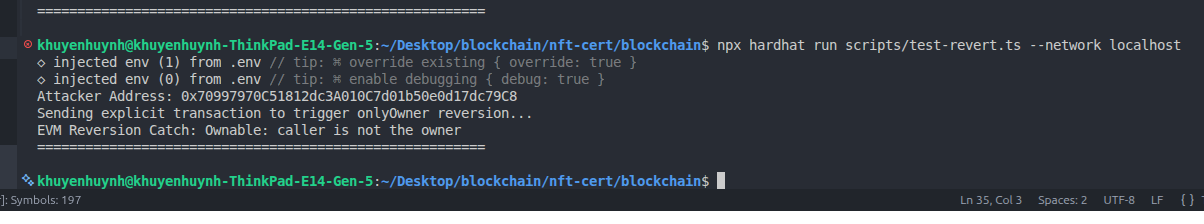
\includegraphics[width=0.85\textwidth]{images/simulate_attack.png}
    \caption{EVM Transaction Reversion Terminal Log}
    \label{fig:simulate_attack}
\end{figure}

\subsubsection{Duplicate Certificate Prevention}

\textbf{1. Threat Model and Collision Attack Vector}\\

The value of an academic degree on a public ledger stems entirely from its uniqueness and non-fungibility \cite{fairfield2022tokenized}. In a flawed implementation, a compromised academic administrator or an attacker exploiting an edge case could attempt a Reissue or Duplicate Mint Attack \cite{perez2020smartcontracts}.The Attacker's Objective:

\begin{itemize}
    \item To reissue an identical certificate payload twice, assigning the duplicate credential to a different student address \cite{khati2023studentcert}.

    \item To artificially inflate graduation metrics or counterfeit credentials by copying a legitimate student's IPFS metadata profile \cite{kumutha2021blockchainacdaemic}.
\end{itemize}

Because metadata hashes (such as IPFS CIDs) are stored as public records on-chain, any network participant can read a valid certificate payload \cite{benet2014ipfs}. If the smart contract state machine only relies on an incremental token counter (e.g., \_nextTokenId++) without anchoring the cryptographic hash of the file to a uniqueness check, the EVM will happily process the transaction \cite{onlinev0835web}. This would create two distinct Token IDs pointing to the exact same academic file hash, permanently damaging the ledger's authority \cite{blockchainineducation}.\\

\textbf{2. Solution: Architectural Implementation of State Uniqueness Checks}\\

To permanently eliminate this attack vector, the smart contract registers every single file hash into a global lookup mapping state variable during execution: \texttt{mapping(string => uint256) private hashToTokenId;} \cite{onlinev0835web}.Before executing the underlying ERC-721 minting routine, the contract evaluates the incoming payload using a strict validation constraint \cite{openzeppelin2026erc721}:

\begin{lstlisting}[
        language=solidity,
        style=codeStyle
    ]
    // Cryptographic uniqueness verification gate
    require(
        hashToTokenId[fileHash] == 0, 
        "A certificate with this file hash already exists"
    );
\end{lstlisting}

When a certificate is minted for the first time, its IPFS file hash does not exist in the mapping, returning the default storage value of 0 \cite{onlinev0835web}. The condition passes, and the contract writes the new Token ID into that slot. If anyone attempts to pass the exact same string (\texttt{fileHash}) again, the mapping evaluates to an integer greater than zero \cite{nfterc721web}. The require statement instantly catches the collision, short-circuits the stack execution, and throws a clear exception string \cite{perez2020smartcontracts}.\\

\textbf{3. Result and State Reversion}\\

This structural pattern guarantees that a duplicate NFT certificate is cryptographically impossible to generate within the ecosystem \cite{wang2021nft}.

\begin{itemize}
    \item EVM Reversion: The transaction fails atomically \cite{wood2008EthereumYellowPaper}. No gas is wasted on computing secondary storage changes, and the network immediately rejects the block \cite{gasandfeesetheweb}.

    \item Database Synchronization Integrity: Because the transaction reverts at the protocol layer, the backend listener fails to capture a Transfer event \cite{ether2026ether}. This prevents any corrupted data state from being mirrored to your off-chain MongoDB instance or local cache pipelines \cite{hardhat2026ethereum}.

    \item Immutable Security Proof: The system achieves a strict 1:1 invariant relationship between a physical academic achievement and its digital blockchain anchor \cite{muhamed2018eductx}.
\end{itemize}

\begin{figure}[H]
    \centering
    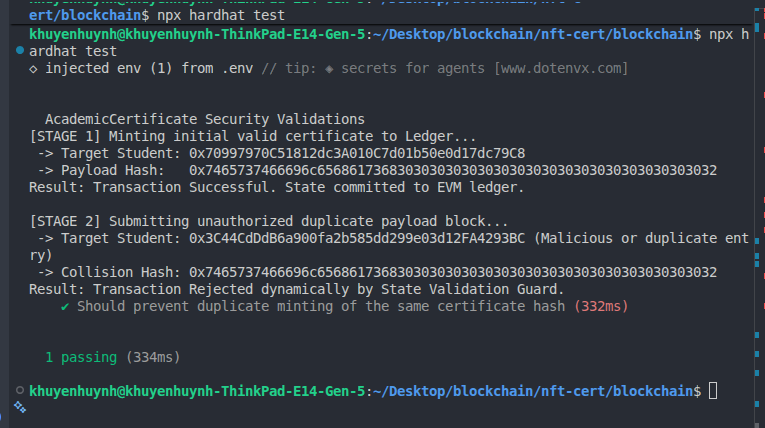
\includegraphics[width=0.85\textwidth]{images/simulate_duplicate.png}
    \caption{Hardhat Test Terminal Catching Duplicate Hash Rejection}
    \label{fig:simulate_duplicate}
\end{figure}

\subsubsection{Soulbound Enforcement}

\textbf{1. The Vulnerability of Standard ERC-721 Tokenization in Academic Credentials}\\

The standard tokenization framework defined by the Ethereum Improvement Proposal (EIP-721) was originally engineered to facilitate the friction-free exchange of digital assets, collectible items, and financial instruments across decentralized networks \cite{fairfield2022tokenized}. To support these secondary liquid markets, the default OpenZeppelin ERC-721 baseline implementation exposes global, publicly accessible state-changing methods, specifically:

\begin{itemize}
    \item \texttt{transferFrom(address from, address to, uint256 tokenId)}

    \item \texttt{safeTransferFrom(address from, address to, uint256 tokenId, bytes data)}
\end{itemize}

While these native features are ideal for tradeable assets, they present a fundamental architectural vulnerability when directly applied to institutional certification ecosystems \cite{blockchainineducation}. Academic degrees, professional licenses, and graduation certificates are intrinsically tied to an individual's unique identity, historical achievement, and verified merit \cite{kumutha2021blockchainacdaemic}. If a university issues a diploma as a vanilla ERC-721 token, the recipient (Student A) retains full cryptographic custody over that asset's state transitions \cite{perez2020smartcontracts}. \\

Consequently, Student A could execute an unauthorized secondary transfer, sending the token to Student B via a direct peer-to-peer transaction or listing it on a public decentralized marketplace (such as OpenSea) for financial gain. This loophole would allow bad actors to purchase, sell, or illicitly inherit authentic academic credentials, entirely breaking the trust assumptions, systemic authority, and verification integrity of the decentralized ledger \cite{khati2023studentcert}.\\

\textbf{2. Architectural Design of Soulbound Tokens (SBTs)}\\

To neutralize this exploit vector and enforce absolute immutability over credential ownership, the system design mutates the standard token layout into a Soulbound Token (SBT) infrastructure \cite{gasandfeesetheweb}. A Soulbound Token is conceptually defined as a non-transferable, identity-anchored digital asset bound permanently to a specific ledger account address (the "Soul") from the exact millisecond of its initial generation \cite{muhamed2018eductx}.\\

The core technical challenge in creating an SBT within an EVM runtime environment involves overriding the asset’s internal state-transition rules without breaking downstream read-only compatibility with mainstream Web3 block explorers (such as Etherscan) or decentralized indexing protocols (such as The Graph) \cite{nfterc721web}. To achieve this, the underlying smart contract overrides the native internal hook mechanics of the ERC-721 standard library, cutting off all transfer execution logic at the protocol layer before any storage changes can be written to the block \cite{onlinev0835web}.\\

\textbf{3. OpenZeppelin v4 Smart Contract Override Implementation}\\

In OpenZeppelin v4 contract configurations, all public-facing transfer functions inside the standard library route their core state updates through an internal execution lifecycle hook called \texttt{\_beforeTokenTransfer}. By intentionally overriding this hook method and placing a conditional validation gate inside its block, we intercept every single asset transfer attempt made across the network \cite{openzeppelin2026erc721}.

\begin{lstlisting}[
        language=solidity,
        style=codeStyle
    ]
    function _beforeTokenTransfer(
        address from,
        address to,
        uint256 firstTokenId,
        uint256 batchSize
    ) internal virtual override {
        super._beforeTokenTransfer(from, to, firstTokenId, batchSize);

        // Enforce Soulbound Invariant: Revert if the transaction is a transfer
        require(
            from == address(0),
            "AcademicSBT: Transfer restriction enforced - Credentials are non-transferable"
        );
    }
\end{lstlisting}


Let's explain the code:
\begin{itemize}
    \item \textbf{The Minting Exception}: When the university administrator triggers \path{mintCertificate()}, the token transits from the non-existent state (\texttt{address(0)}) to the target student’s wallet. The contract evaluates \texttt{from == address(0)}, which returns true. The validation check passes cleanly, and the initialization function completes successfully \cite{onlinev0835web}.

    \item \textbf{The Transfer Block}: If any actor later attempts to call \path{transferFrom()} or \path{safeTransferFrom()}, the internal state engine routes the data stream into this overridden hook before updating the token's registry mappings \cite{nfterc721web}. The parameter from evaluates to the student's current wallet address (which is not \texttt{address(0)}). The \texttt{require} constraint instantly fails, intercepts the call stack, throws an exception string, and triggers an absolute state reversion \cite{ether2026ether}.
\end{itemize}

\textbf{4. Structural Data Flow and Rejection Mechanics}\\

The diagram below maps the complete lifecycle of a blocked transfer transaction under the OpenZeppelin v4 architecture. When a user or a third-party script triggers a transfer payload, the transaction is pushed to the local EVM node where the runtime memory space isolates the execution failure, cancels the transaction pipeline, and preserves the original ownership state perfectly.

\begin{figure}[H]
    \centering
    \begin{tikzpicture}[
            font=\small,
            node distance=1.8cm,
            block/.style={
                    rectangle,
                    draw,
                    thick,
                    text width=6.5cm,
                    align=center,
                    rounded corners=2pt,
                    minimum height=1cm
                },
            hookblock/.style={
                    rectangle,
                    draw,
                    thick,
                    text width=7cm,
                    align=left,
                    rounded corners=2pt,
                    inner sep=8pt
                },
            revertblock/.style={
                    rectangle,
                    draw,
                    thick,
                    text width=6.5cm,
                    align=center,
                    rounded corners=2pt,
                    minimum height=0.8cm
                },
            line/.style={draw, thick},
            labelstyle/.style={align=left, font=\scriptsize, inner sep=2pt}
        ]

        \node [block] (registry) {
            \textbf{University Registry}
        };

        \node [block, below=of registry] (studentA) {
            \textbf{Student A} \\
            \footnotesize(0x70997970C51812dc3A010C7d01....)
        };

        \node [hookblock, below=of studentA] (hook) {
            \textbf{OpenZeppelin v4 Lifecycle Hook} \\
            \rule{\linewidth}{0.4pt} \\
            \textbf{Invokes:} \texttt{\_beforeTokenTransfer()} \\
            \textbf{Checks:} \texttt{from == address(0)} (\textit{Evaluates to False})
        };

        \node [revertblock, below=of hook] (revert) {
            \textbf{REJECTED} \\
            \footnotesize {Reason: "Transfer restriction enforced"}
        };

        \node [block, below=of revert] (studentB) {
            \textbf{Student B} \\
            \footnotesize(0x3C44CdDdB6a900fa2b585dd299e...) \\
            \vspace{2pt}
            \scriptsize\textit{(Result: Receives 0x0 Tokens / State Unchanged)}
        };

        \path [line, ->] (registry) -- node[labelstyle, midway, right] {1. \texttt{mintCertificate()}} (studentA);

        \path [line, ->] (studentA) -- node[labelstyle, midway, right] {2. Attempts P2P Transfer\\ \hspace*{10pt}via \texttt{transferFrom()}} (hook);

        \path [line, ->] (hook) -- node[labelstyle, midway, right] {3. TRANSACTION REVERTED} (revert);

        \path [line, ->, dashed, draw] (revert) -- (studentB);

    \end{tikzpicture}
    \caption{Lifecycle of a blocked transfer transaction}
    \label{fig:sbt_lifecycle}
\end{figure}


\subsubsection{Hash Tampering Protection}

\textbf{1. Cryptographic Hashing and Data Integrity}\\

To protect certificate integrity, the proposed system uses the SHA-256 cryptographic hash algorithm \cite{fairfield2022tokenized}. A hash function converts an input file into a fixed-length 256-bit value, commonly represented as a 64-character hexadecimal string \cite{openzeppelin2026erc721}.\\

In this system, the generated hash acts as a digital fingerprint of the certificate. Even a very small modification to the document, such as changing a single character or punctuation mark, produces a completely different hash value. This property is known as the \textit{Avalanche Effect} \cite{blockchainineducation}. In a secure hashing algorithm, a minute modification to the input dataset—even a single bit flip or changing a single punctuation mark inside an academic transcript—will cause a cascade of changes throughout the calculation steps. As a result, the final output hex string changes completely and unpredictably, bearing no statistical correlation to the original hash string \cite{nfterc721web}. The mathematical properties of this protection architecture include:

\begin{itemize}
    \item \textbf{Pre-image Resistance}: Given a target hash $H$, it is computationally impossible to reconstruct the original certificate file contents $x$ such that $\text{SHA-256}(x) = H$ \cite{muhamed2018eductx}.
    \item \textbf{Collision Resistance}: It is extremely difficult to find two distinct certificate files that generate the exact same output hash signature \cite{onlinev0835web}.
    \item \textbf{Deterministic Execution}: The identical certificate file will always yield the exact same 64-character hex signature, allowing for decentralized verification without a central authority \cite{gasandfeesetheweb}.
\end{itemize}

\textbf{2. Certificate Tampering Scenario}\\

In traditional digital credential systems, an attacker or a dishonest student can easily manipulate PDF documents using standard editing software \cite{kumutha2021blockchainacdaemic}. For example, a student might modify their GPA from \texttt{2.8} to \texttt{3.8}, or alter the text inside the major field from \texttt{Computer Science} to \texttt{Artificial Intelligence} \cite{perez2020smartcontracts}. Since standard PDF files do not natively contain an immutable tamper-evident validation layer, these changes are hard to detect unless a verifier manually contacts the issuing university registry \cite{khati2023studentcert}. Within our decentralized platform, when a university issues a degree, the system executes a dual-anchoring sequence:

\begin{itemize}
    \item The complete structured student profile metadata is written to the InterPlanetary File System (IPFS) \cite{benet2014ipfs}.

    \item The raw, original binary array of the physical certificate PDF file (Certificate.pdf) is hashed locally inside the client browser interface using SHA-256 to generate a unique digital fingerprint, which is passed directly to the smart contract’s fileHash state variable \cite{onlinev0835web}.
\end{itemize}

If a student attempts to upload a modified PDF file to a validation portal, the verification engine dynamically computes the SHA-256 signature of the uploaded file on-the-fly and compares it against the immutable hashToTokenId tracking mapping recorded on the blockchain ledger \cite{nfterc721web}.\\

\textbf{3. Demonstration: The Impact of Single-Character Manipulation}\\

To demonstrate the sensitivity of the system's tamper-detection mechanism, The below table tracks the output values generated when a standard degree certificate payload undergoes minor unauthorized modifications.

\begin{longtable}{|m{2.8cm}|m{4.0cm}|m{4.0cm}|m{2.5cm}|}
    \hline
    \textbf{Scenario}                                                        &
    \textbf{Input Target File (\texttt{Certificate.pdf})}                    &
    \textbf{Computed SHA-256 Hexadecimal Hash Signature}                     &
    \textbf{System Verification Status}                                        \\
    \hline
    \endfirsthead

    Baseline                                                                 &
    \path{Name: Nguyen Thi Hoa, Major: Software Engineering, ...., GPA: 2.3} &
    \path{8b5a1f6c4d2e...3e7f9a0b1c2}                                        &
    VALID                                                                      \\
    \hline

    Tamper Attempt 1                                                         &
    \path{Name: Nguyen Thi Hoa, Major: Software Engineering, ...., GPA: 3.2} &
    \path{4f7e2a1b9c0d...a6b7c8d9e0f}                                        &
    REJECTED (Hash Mismatch)                                                   \\
    \hline

    Tamper Attempt 2                                                         &
    \path{Name: Nguyen Thi Hoa, Major: Software EngineerinG, ...., GPA: 3.8} &
    \path{c9a1b2c3d4e5...f6a7b8c9d0e}                                        &
    REJECTED (Hash Mismatch)                                                   \\
    \hline

    \caption{SHA-256 Output Variance Tracing via Minor Payload Alterations}
    \label{tab:attempt_modify}                                                 \\
\end{longtable}

As shown in the evaluation metrics above, changing a single decimal point in the GPA string (from 2.3 to 3.2) or changing a single lowercase character to uppercase (Engineering to EngineerinG) creates an entirely different cryptographic signature \cite{blockchainineducation}. The new signature bears no structural resemblance to the baseline hash value registered on-chain.\\

\textbf{4. Dynamic Verification Logic and Rejection Mechanics}\\

When a third-party verifier (such as a recruiter or a corporate employer) drops a certificate PDF onto the verification portal interface, the system executes the following verification pipeline \cite{hardhat2026ethereum}:

$$\text{Verification Status} = \begin{cases}
        \text{Success}, & \text{if } \text{hashToTokenId}[\text{SHA-256}(\text{Uploaded File})] > 0 \\
        \text{Failure}, & \text{if } \text{hashToTokenId}[\text{SHA-256}(\text{Uploaded File})] = 0
    \end{cases}$$


If any data has been tampered with, the lookup mapping searches for the altered hash variant string (\texttt{XYZ999...}) instead of the true record string (\texttt{ABCD123...}) \cite{onlinev0835web}. Because the altered hash string has never been initialized by the onlyOwner institutional minting routine, the EVM lookup evaluates to its default uninitialized integer value: 0 \cite{nfterc721web}. The client web application captures this null index response, flags the asset as a forged credential, and updates the user interface with a clear warning notification \cite{hardhat2026ethereum}. This design pattern completely eliminates credential forgery. An attacker cannot alter a single byte of their academic document without instantly breaking the underlying cryptographic proof, ensuring absolute security across the ecosystem \cite{muhamed2018eductx}.

\subsubsection{Wallet Ownership Security}

\textbf{1. The Paradigm of Self-Sovereign Identity and Ledger Ownership}\\

In traditional centralized enterprise applications, user accounts, data profiles, and access permissions are managed by a central database administrator using standard authentication systems (such as username/password pairs or OAuth tokens) \cite{hardhat2026ethereum}. Under that legacy framework, users do not own their identity data; they are merely granted access to a database row that can be modified, revoked, or compromised by a central authority or database breach.\\

Our decentralized platform shifts this paradigm to a Self-Sovereign Identity (SSI) and cryptographic ownership model \cite{kumutha2021blockchainacdaemic}. Within this architecture, an academic degree or certificate is not an arbitrary row in an institutional database. Instead, it is an independent digital asset (a Soulbound NFT) permanently mapped to a specific, unique cryptographic wallet address on the blockchain ledger \cite{fairfield2022tokenized}. The ownership of this asset is strictly governed by asymmetric cryptography, where the student's wallet address acts as a public identifier, and access control is enforced entirely by the corresponding mathematical private key \cite{muhamed2018eductx}.\\

\textbf{2. The Cryptographic Asymmetry: Public Addresses vs. Private Keys}\\

The security of an individual's academic credential portfolio relies on the mathematical relationship between two keys generated via the Elliptic Curve Digital Signature Algorithm (ECDSA), specifically the \texttt{secp256k1} curve standard used by Ethereum-compatible networks \cite{nfterc721web}:

\begin{enumerate}
    \item The Public Key / Wallet Address ($A_{pub}$): This is a 20-byte (160-bit) hexadecimal string derived from the student's public key (e.g., \texttt{0x7099...79C8}). It acts as a public identity anchor. The smart contract maps the issued Token ID directly to this address inside its internal ownership registry: \texttt{mapping(uint256 => address) private \_owners;} \cite{onlinev0835web}.
    \item The Private Key ($k_{priv}$): This is a secret 256-bit randomly generated integer that is kept entirely confidential by the student (usually managed securely inside an isolated hardware module or a non-custodial software wallet like MetaMask) \cite{blockchainineducation}.
\end{enumerate}

Because the token is structurally bound to the wallet address, only the holder of the matching private key can interact with or prove ownership of that specific academic degree \cite{perez2020smartcontracts}. The private key is mathematically required to generate a valid cryptographic signature ($\sigma$) for any outbound transaction or off-chain verification challenge \cite{openzeppelin2026erc721}. Without access to this private key, it is computationally impossible for an outside attacker to forge a signature or impersonate the credential holder, ensuring absolute security across the ecosystem \cite{muhamed2018eductx}.\\

\textbf{3. Smart Contract Access Control and Institutional Isolation}\\

To protect the student from unauthorized delegation, credential theft, or accidental listings on secondary marketplaces, the \texttt{AcademicCertificate} contract explicitly intercepts token custody state changes using internal lifecycle overrides from the base OpenZeppelin ERC-721 library \cite{gasandfeesetheweb}.

Rather than solely masking user-facing methods, the contract establishes a foundational execution constraint at the core token transfer pipeline. This architectural strategy guarantees that any high-level transfer invocation instantly reverts unless it is part of the initial minting routine:

\begin{lstlisting}[
        language=solidity,
        style=codeStyle
    ]
    function _beforeTokenTransfer(
        address from,
        address to,
        uint256 firstTokenId,
        uint256 batchSize
    ) internal virtual override {
        super._beforeTokenTransfer(from, to, firstTokenId, batchSize);

        require(
            from == address(0),
            "AcademicSBT: Transfer restriction enforced - Credentials are non-transferable"
        );
    }

    function approve(address, uint256) public pure override {
        revert("Soulbound: No approvals allowed");
    }

    function setApprovalForAll(address, bool) public pure override {
        revert("Soulbound: No approvals allowed");
    }
\end{lstlisting}

\begin{itemize}
    \item \textbf{Lifecycle Hook Interception}: Intercepting the internal \texttt{\_beforeTokenTransfer} loop creates a centralized validation point. Because token minting operations route through this identical sequence, the logical assertion evaluates the source address parameter. If the \texttt{from} state is not the zero-address (\texttt{address(0)}), the system recognizes the transaction as an impermissible secondary market move or peer-to-peer exchange and forcefully terminates execution \cite{nfterc721web}.

    \item \textbf{Exploitation Surface Mitigation}: While the internal hook stops actual token movement, the public interface explicitly overrides \texttt{approve()} and \texttt{setApprovalForAll()}. Uniquely, these are declared with the \texttt{pure} visibility modifier since their execution blocks immediately call \texttt{revert()} without reading or writing to the underlying contract state. This proactively neutralizes third-party market listings before any transactional payloads hit the state machine \cite{nfterc721web}.

    \item \textbf{Deterministic Collision Resistance}: To maintain rigorous document validation standards, the minting mechanism tracks document uniqueness using a strict state mapping: \\
          \path{mapping(string => uint256) public hashToTokenId;}. \\
          Before a token is securely allocated, the contract evaluates whether \path{hashToTokenId[fileHash] == 0}. This prevents an administrative error or threat actor from duplicate-minting an identical cryptographic file signature onto multiple distinct token IDs \cite{nfterc721web}.

    \item \textbf{Institutional Isolation}: Furthermore, administrative controls are tightly sandboxed using the standard OpenZeppelin \texttt{onlyOwner} modifier \cite{perez2020smartcontracts}. While the university registry maintains exclusive authorization to invoke \texttt{mintCertificate()} and \texttt{revokeCertificate()}, it holds no operational control or recovery vector to manipulate or alter a certificate once it is cryptographically anchored to a student's public address \cite{onlinev0835web}.
\end{itemize}

\textbf{4. Structural Authentication and Ownership Verification Flow}\\

The diagram below maps how the system verifies wallet ownership. When a student attempts to access their profile or present their credentials to a verification portal, the application uses an off-chain cryptographic challenge-response routine (EIP-712) to verify private key ownership without exposing the key itself.

\begin{figure}[H]
    \centering
    \begin{tikzpicture}[
            font=\small,
            >=Stealth,
            headerbox/.style={
                    rectangle,
                    draw,
                    thick,
                    text width=4.8cm,
                    align=center,
                    minimum height=1.2cm,
                    rounded corners=2pt
                },
            gatebox/.style={
                    rectangle,
                    draw,
                    thick,
                    text width=7.5cm,
                    align=left,
                    inner sep=10pt,
                    rounded corners=2pt
                },
            resultbox/.style={
                    rectangle,
                    draw,
                    thick,
                    text width=3.2cm,
                    align=center,
                    minimum height=1.2cm,
                    rounded corners=2pt
                },
            line/.style={draw, thick},
            msgline/.style={draw, ->, thick},
            labelstyle/.style={font=\sffamily\scriptsize, fill=white, inner sep=2pt, align=left}
        ]

        \node [headerbox] (portal) {\textbf{Verification Portal}\\ \footnotesize(Web3 App Interface)};
        \node [headerbox, right=3.5cm of portal] (wallet) {\textbf{Student Client Wallet}\\ \footnotesize(MetaMask / Non-Custodial)};

        \draw [line, dashed, gray] (portal.south) -- +(0, -3.2cm) coordinate (portal_base);
        \draw [line, dashed, gray] (wallet.south) -- +(0, -3.2cm) coordinate (wallet_base);

        \draw [msgline] ($(portal.south)+(0,-0.6cm)$) -- node[labelstyle, midway, yshift=4pt] {
            1. Generates Random Challenge\\
            \texttt{"Sign: Auth\_Session\_2026"}
        } ($(wallet.south)+(0,-0.6cm)$);

        \node [anchor=west, font=\sffamily\scriptsize, text width=4cm, align=left, xshift=5pt] at ($(wallet.south)+(0,-1.7cm)$) {
            2. Approves prompt with\\ \hspace*{10pt}Private Key ($k_{priv}$)\\
            3. Generates Signature ($\sigma$)
        };

        \draw [msgline] ($(wallet.south)+(0,-2.6cm)$) -- node[labelstyle, midway, yshift=4pt] {
            4. Returns Cryptographic Signature ($\sigma$)
        } ($(portal.south)+(0,-2.6cm)$);

        \node [gatebox, below=3.2cm of portal.south, xshift=2.1cm] (gate) {
            \textbf{Cryptographic Validation Gate} \\
            \rule{\linewidth}{0.4pt} \\
            \textbf{Math:} \texttt{ecrecover(Challenge, $\sigma$)} $\rightarrow$ \textit{Returns Address} \\
            \textbf{Query:} Is derived Address == Token Owner?
        };

        \coordinate (gate_bottom) at (gate.south);

        \node [resultbox] (match) at ($(gate_bottom) + (-2.2cm, -2.2cm)$) {
            \textbf{MATCH} \\
            \vspace{2pt}
            \footnotesize Access Granted\\
            \scriptsize (Owner Confirmed)
        };

        \node [resultbox] (mismatch) at ($(gate_bottom) + (2.2cm, -2.2cm)$) {
            \textbf{MISMATCH} \\
            \vspace{2pt}
            \footnotesize Access Denied\\
            \scriptsize (Signature Invalid)
        };

        \draw [line, ->] (gate_bottom) -- +(0,-0.4cm) -| (match.north);
        \draw [line, ->] (gate_bottom) -- +(0,-0.4cm) -| (mismatch.north);

    \end{tikzpicture}
    \caption{Off-Chain Verification Mechanism via Asymmetric ECDSA Challenge-Response Handshake.}
    \label{fig:crypto_verification}
\end{figure}


\textbf{5. Deterministic Security Results}\\

This architectural layout guarantees several deterministic security outcomes for the student's data portfolio:

\begin{itemize}

    \item Immunity to Database Hacks: Because the credentials exist on a decentralized ledger rather than a centralized server, a security breach at the university's IT infrastructure cannot result in the theft, modification, or leakage of already-issued student certificate assets \cite{khati2023studentcert}.

    \item Absolute Asset Custody: The student maintains absolute lifetime custody of their verified achievements \cite{kumutha2021blockchainacdaemic}. No university administrator, corporate entity, or malicious network participant can manipulate the underlying state mappings without possessing the student's unique private key \cite{nfterc721web}.

    \item Phishing and Front-Running Resistance: Since approvals and peer-to-peer transfers are entirely disabled at the internal contract layer, students are completely immune to common Web3 phishing attacks (such as "blind signing" a malicious marketplace approval transaction), ensuring that their academic portfolio remains secure even if they interact with an untrusted decentralized application \cite{blockchainineducation}.

\end{itemize}